\section{Segunda Consigna: Gráficos y Análisis}

\subsection{Resultados}

\subsubsection{Red Laboral}

Con las capturas de esta red, se puede notar la gran cantidad de nodos y trafico de paquetes.
El gráfico de topología era tan extenso que decidimos no ponerlo.

\FloatBarrier

\subsubsection{Histogramas (de IPs y protocolos)}

\begin{figure}[h!]
  \centering
   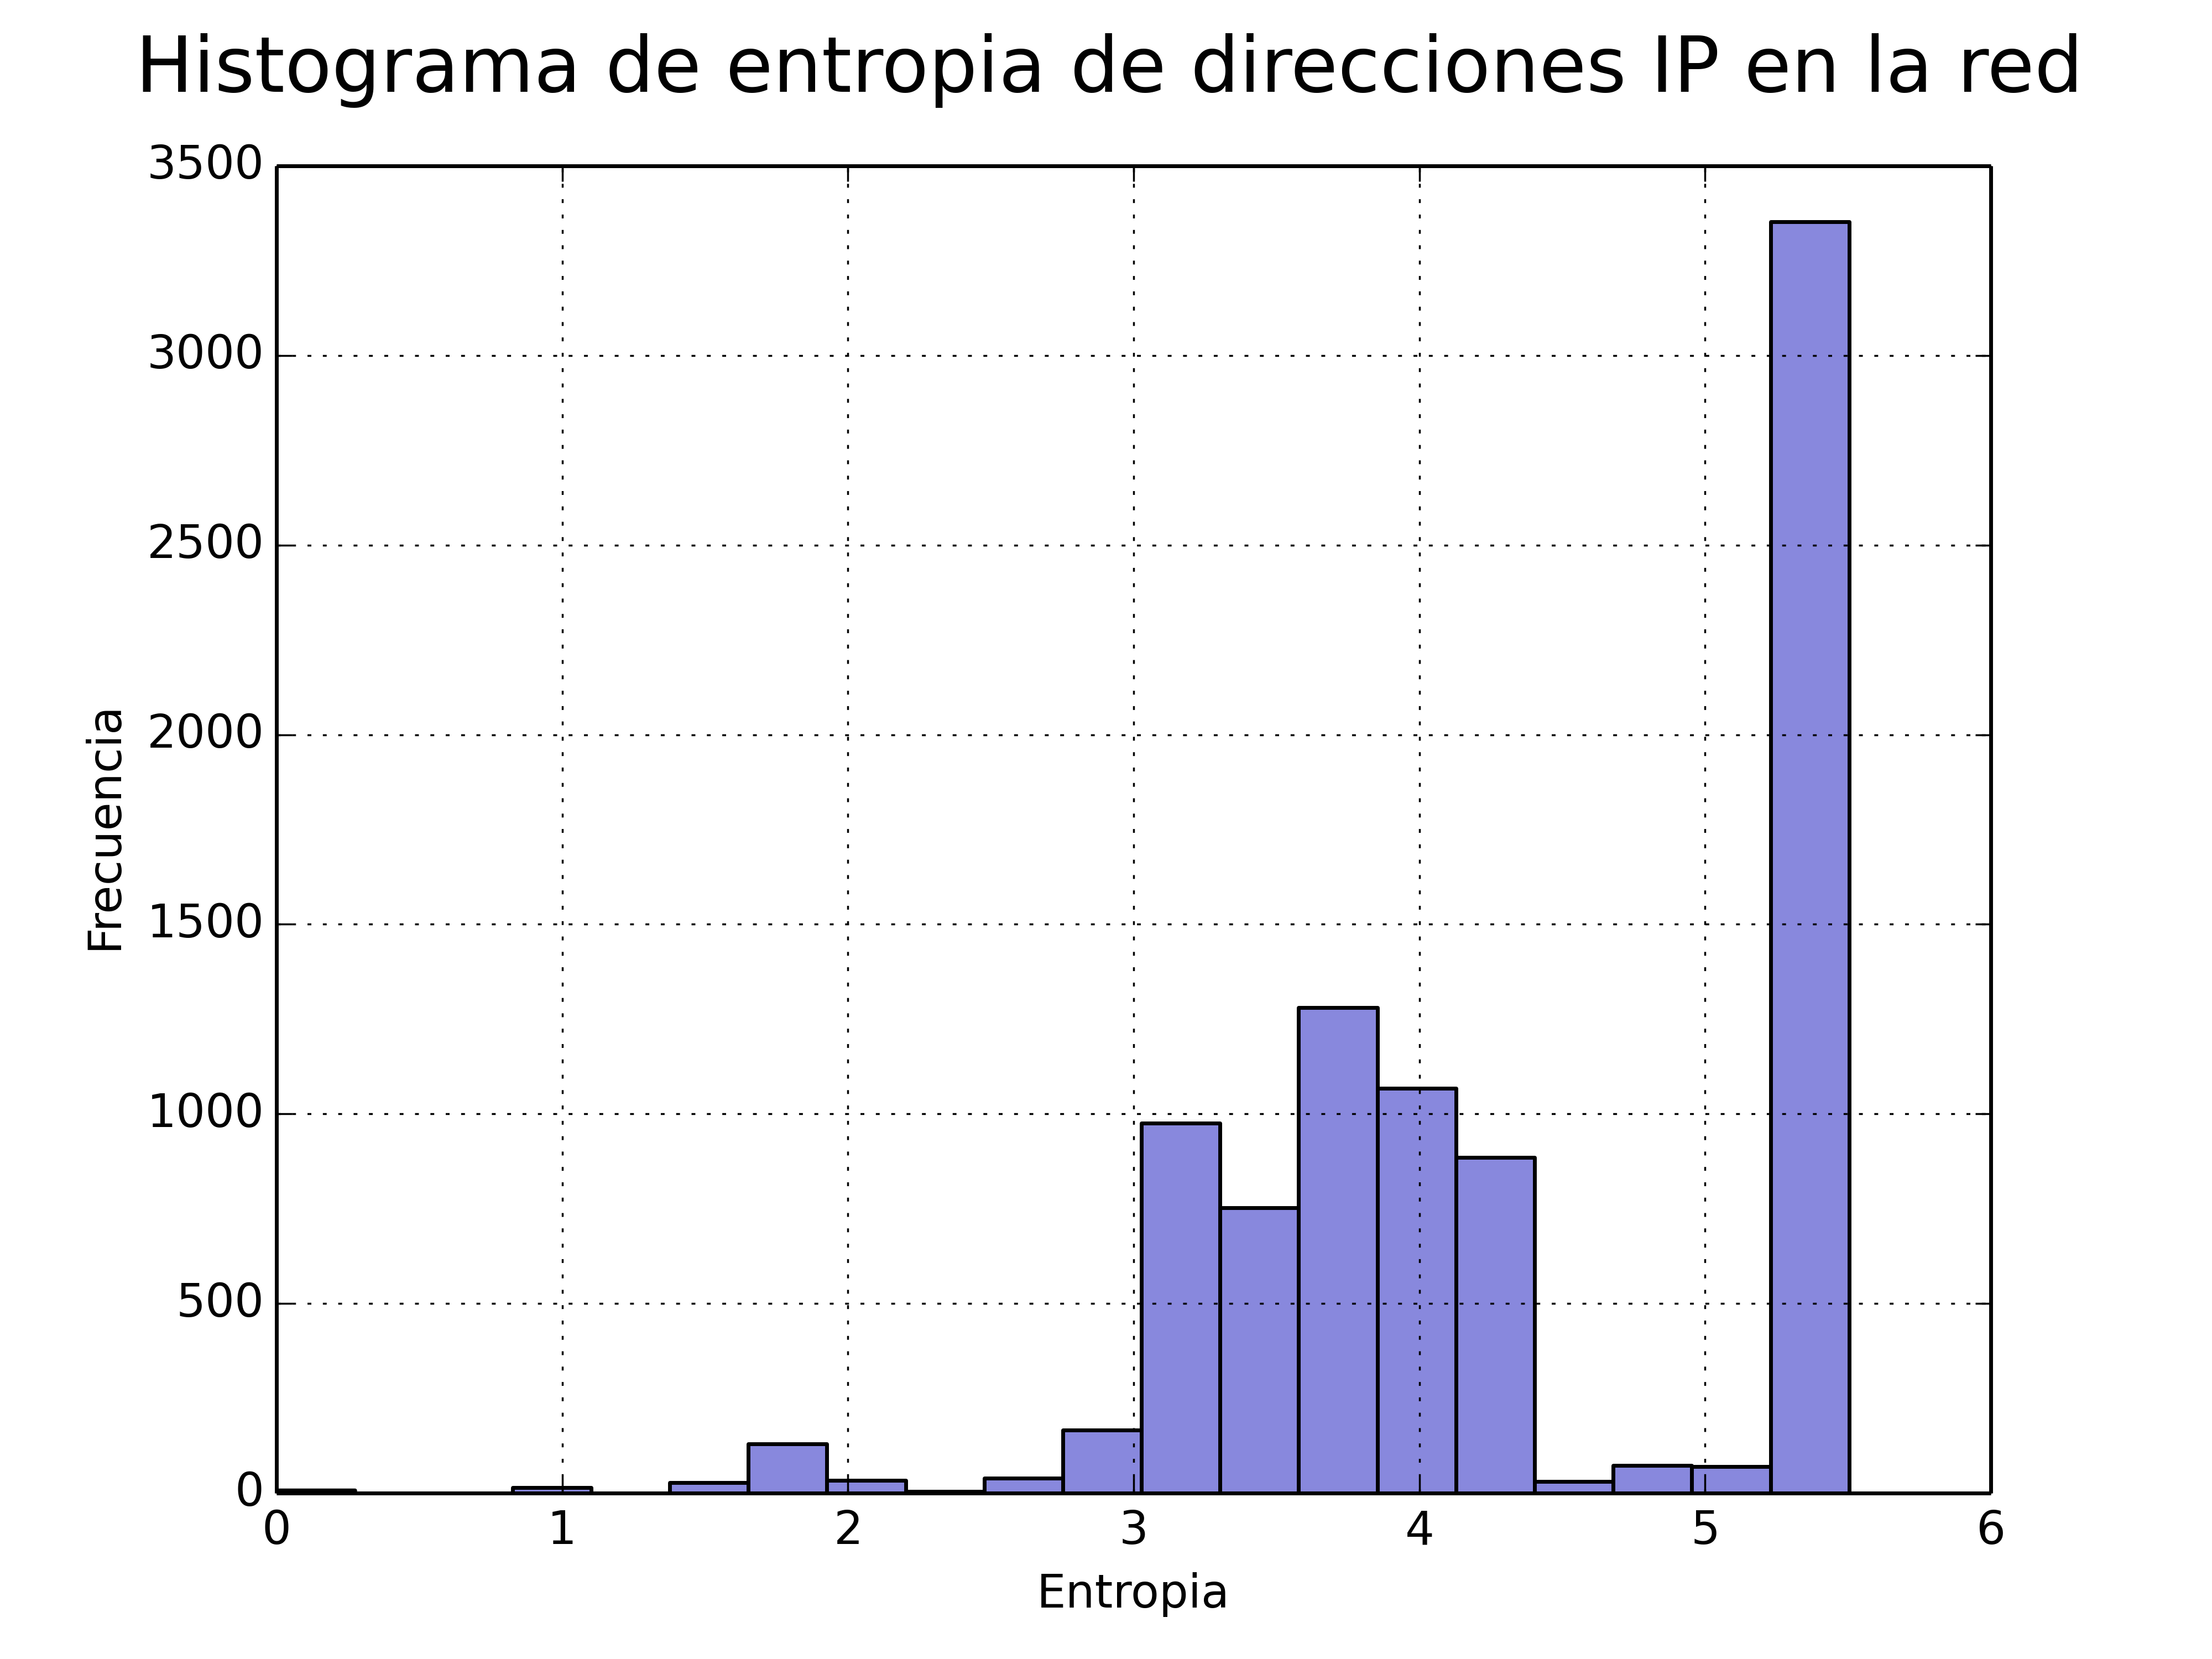
\includegraphics[width=0.7\textwidth]{graficos/red_baufest_hist_arp.png}
  \caption{Mi Figura}
  \label{fig:red_baufest_hist_arp}
\end{figure}

\begin{figure}[h!]
  \centering
   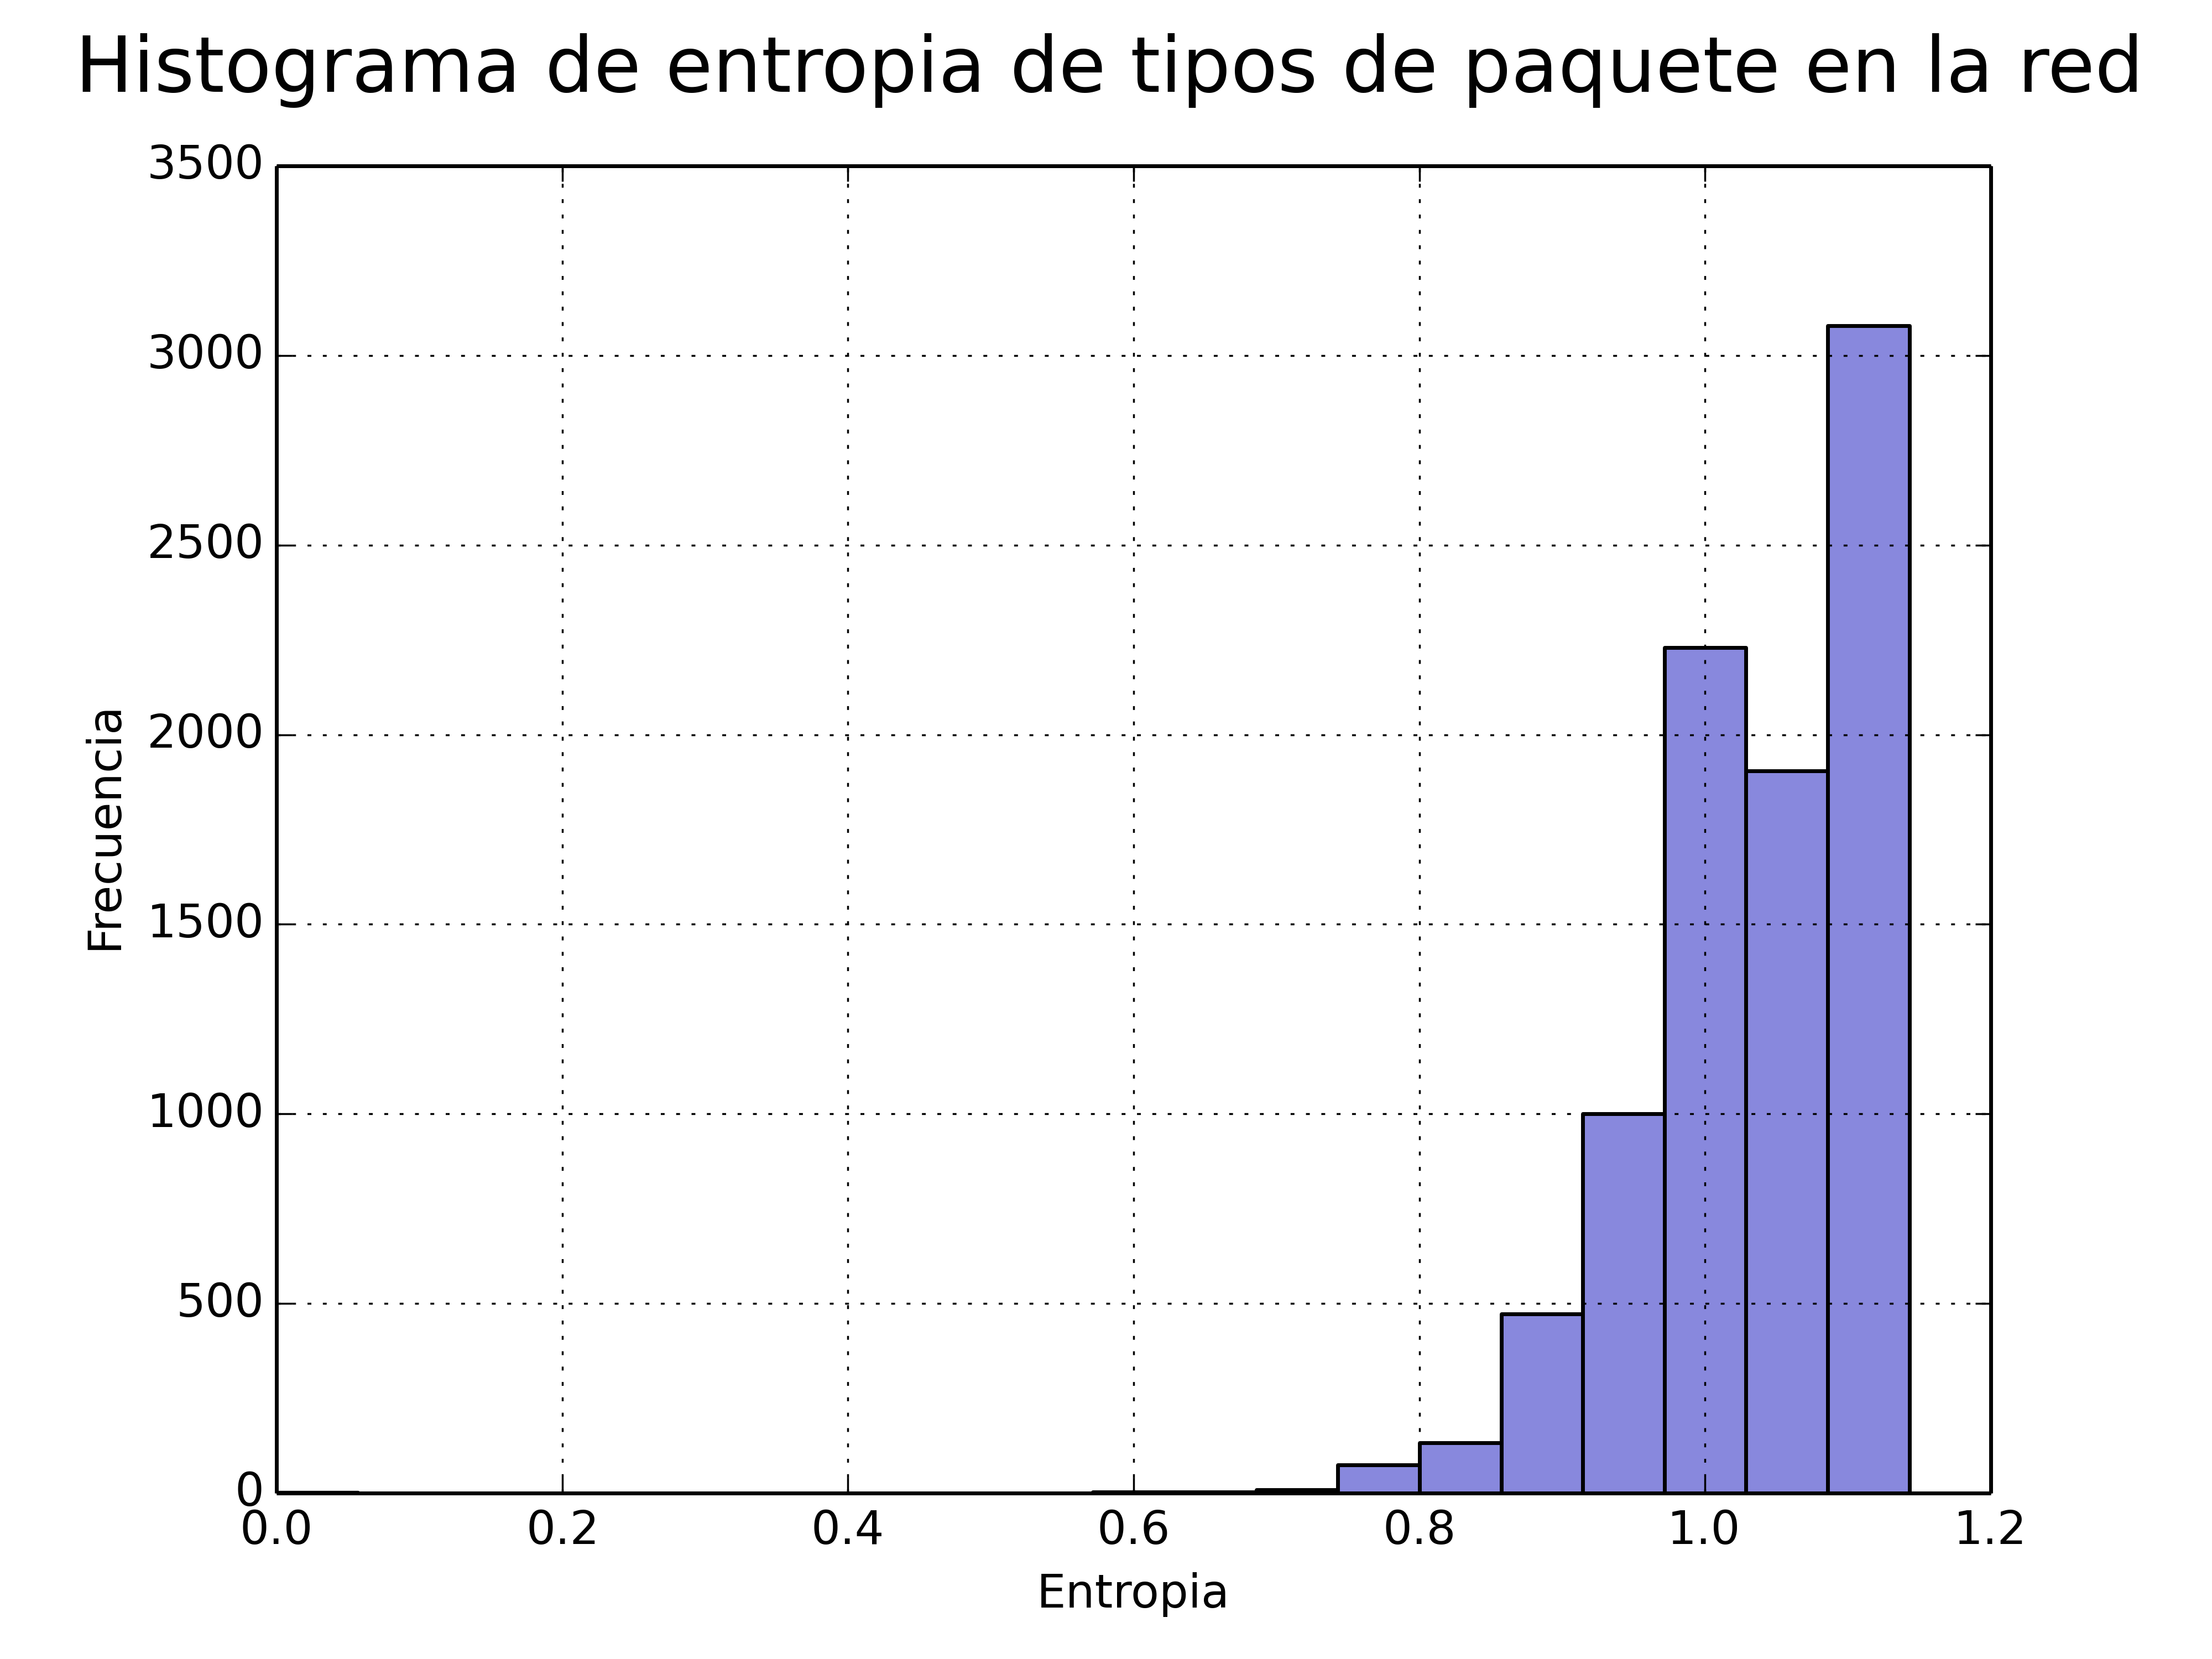
\includegraphics[width=0.7\textwidth]{graficos/red_baufest_hist_type.png}
  \caption{Mi Figura}
  \label{fig:red_baufest_hist_type}
\end{figure}

\FloatBarrier

\subsubsection{Paquetes capturados e información}

Si bien es una red grande, se puede ver en los gráficos que hay 2 nodos que distinguen del resto  192.168.26.43 con el 0.2\% y el 192.168.26.1 con el 0.17\% .
Se presume que esos nodos tienen que ser routers ~\ref{fig:red_baufest_pie_arp} ~\ref{fig:red_baufest_pie_arp_information}. 

En los gráficos de protocolos se vuelve a repetir que el protocolo IP es el mas frecuente. Pero también se observa gran cantidad de paquetes IPv6 ~\ref{fig:red_baufest_pie_type} ~\ref{fig:red_baufest_pie_type_information}. 

\begin{figure}[h!]
  \centering
   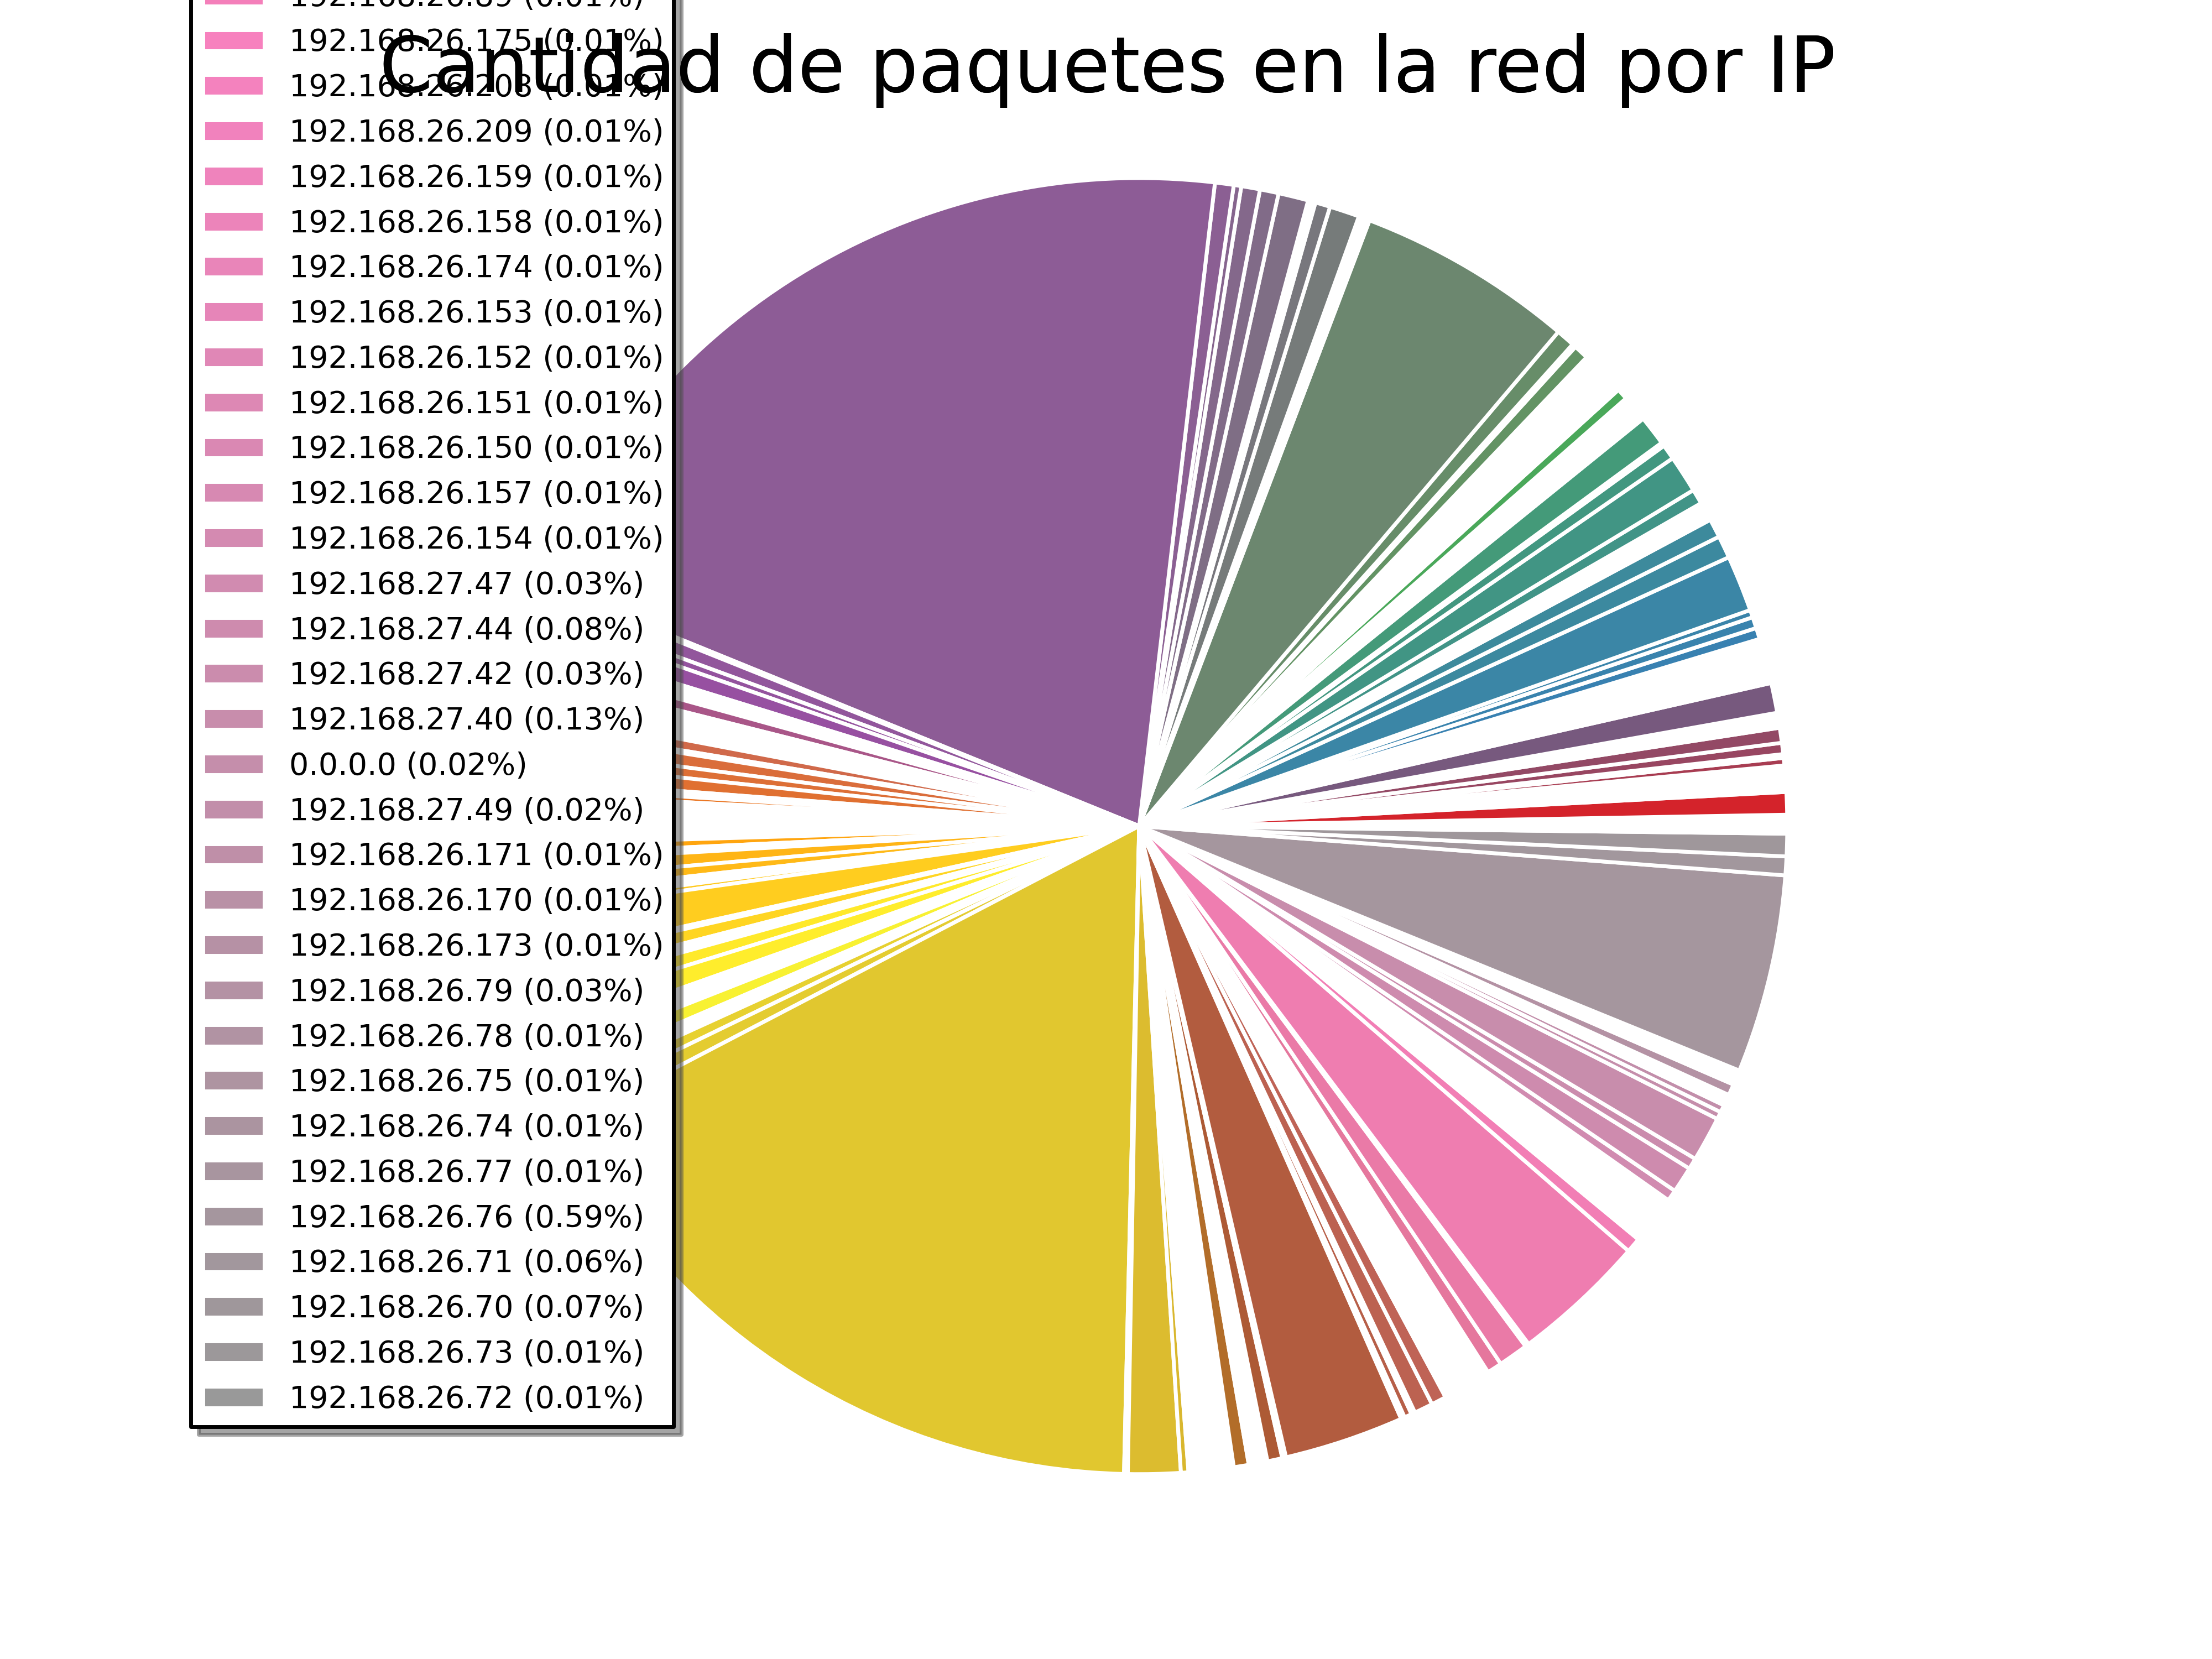
\includegraphics[width=0.7\textwidth]{graficos/red_baufest_pie_arp.png}
  \caption{Mi Figura}
  \label{fig:red_baufest_pie_arp}
\end{figure}

\begin{figure}[h!]
  \centering
   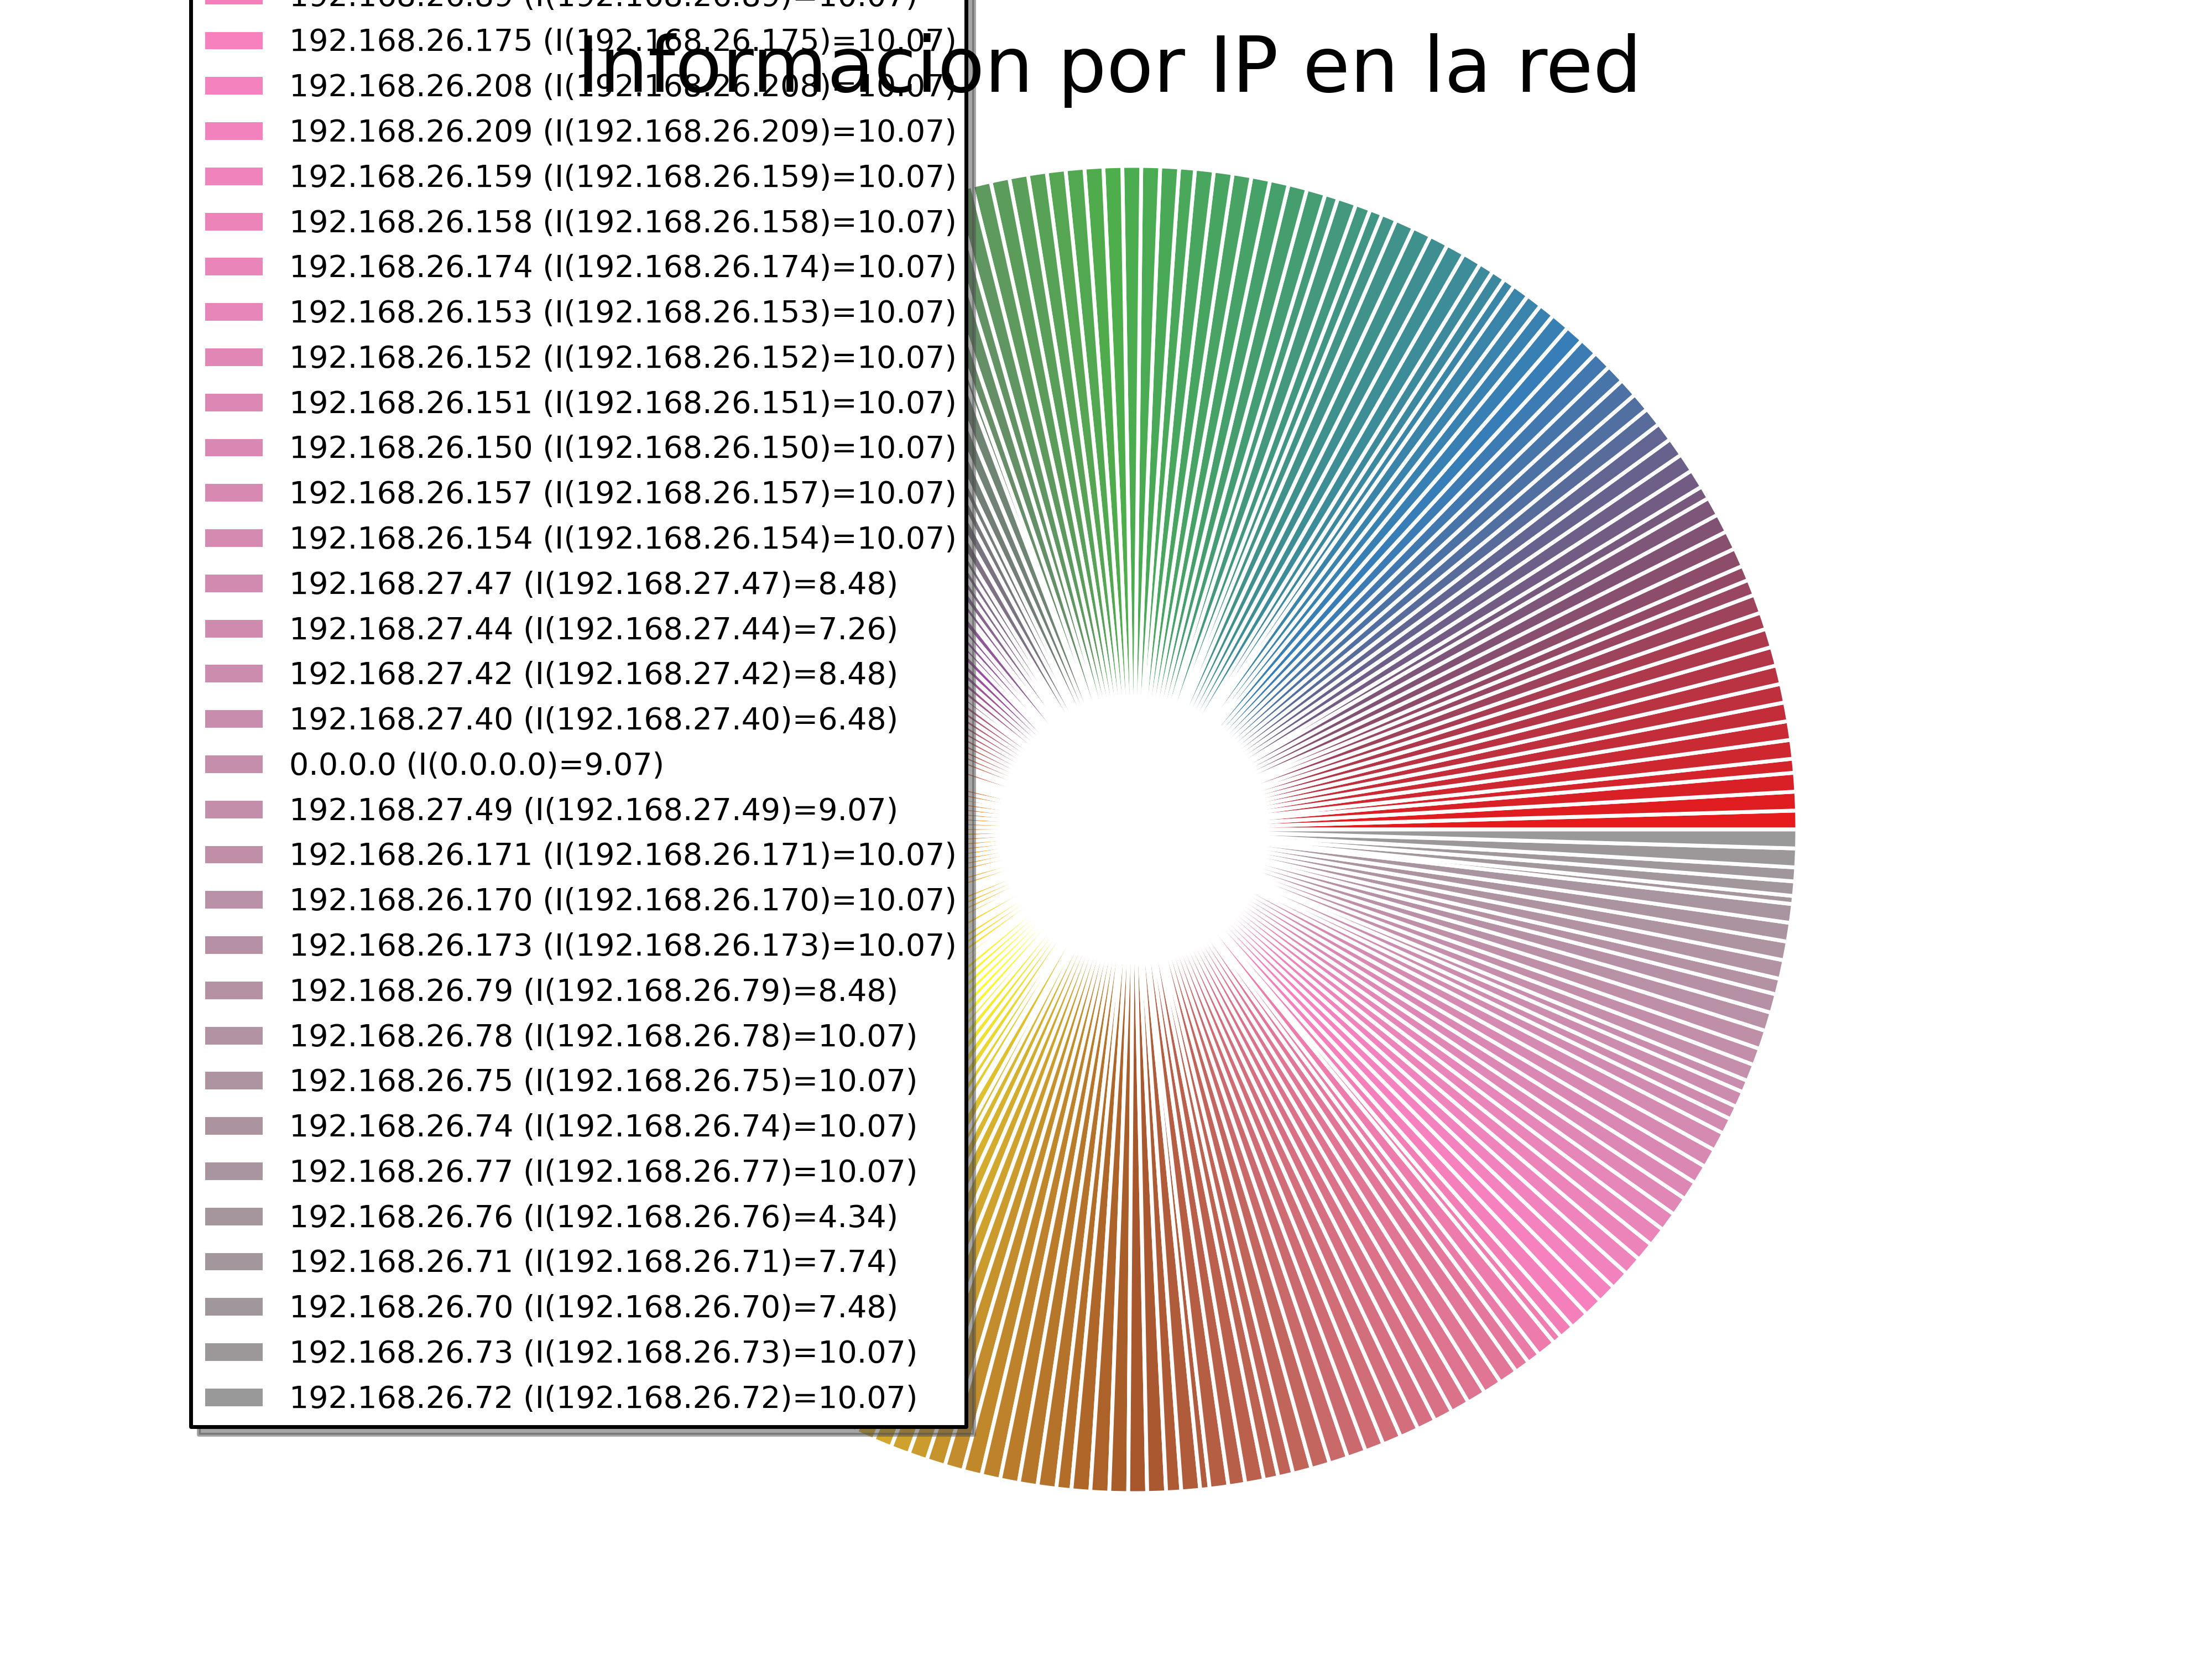
\includegraphics[width=0.7\textwidth]{graficos/red_baufest_pie_arp_information.png}
  \caption{Mi Figura}
  \label{fig:red_baufest_pie_arp_information}
\end{figure}

\begin{figure}[h!]
  \centering
   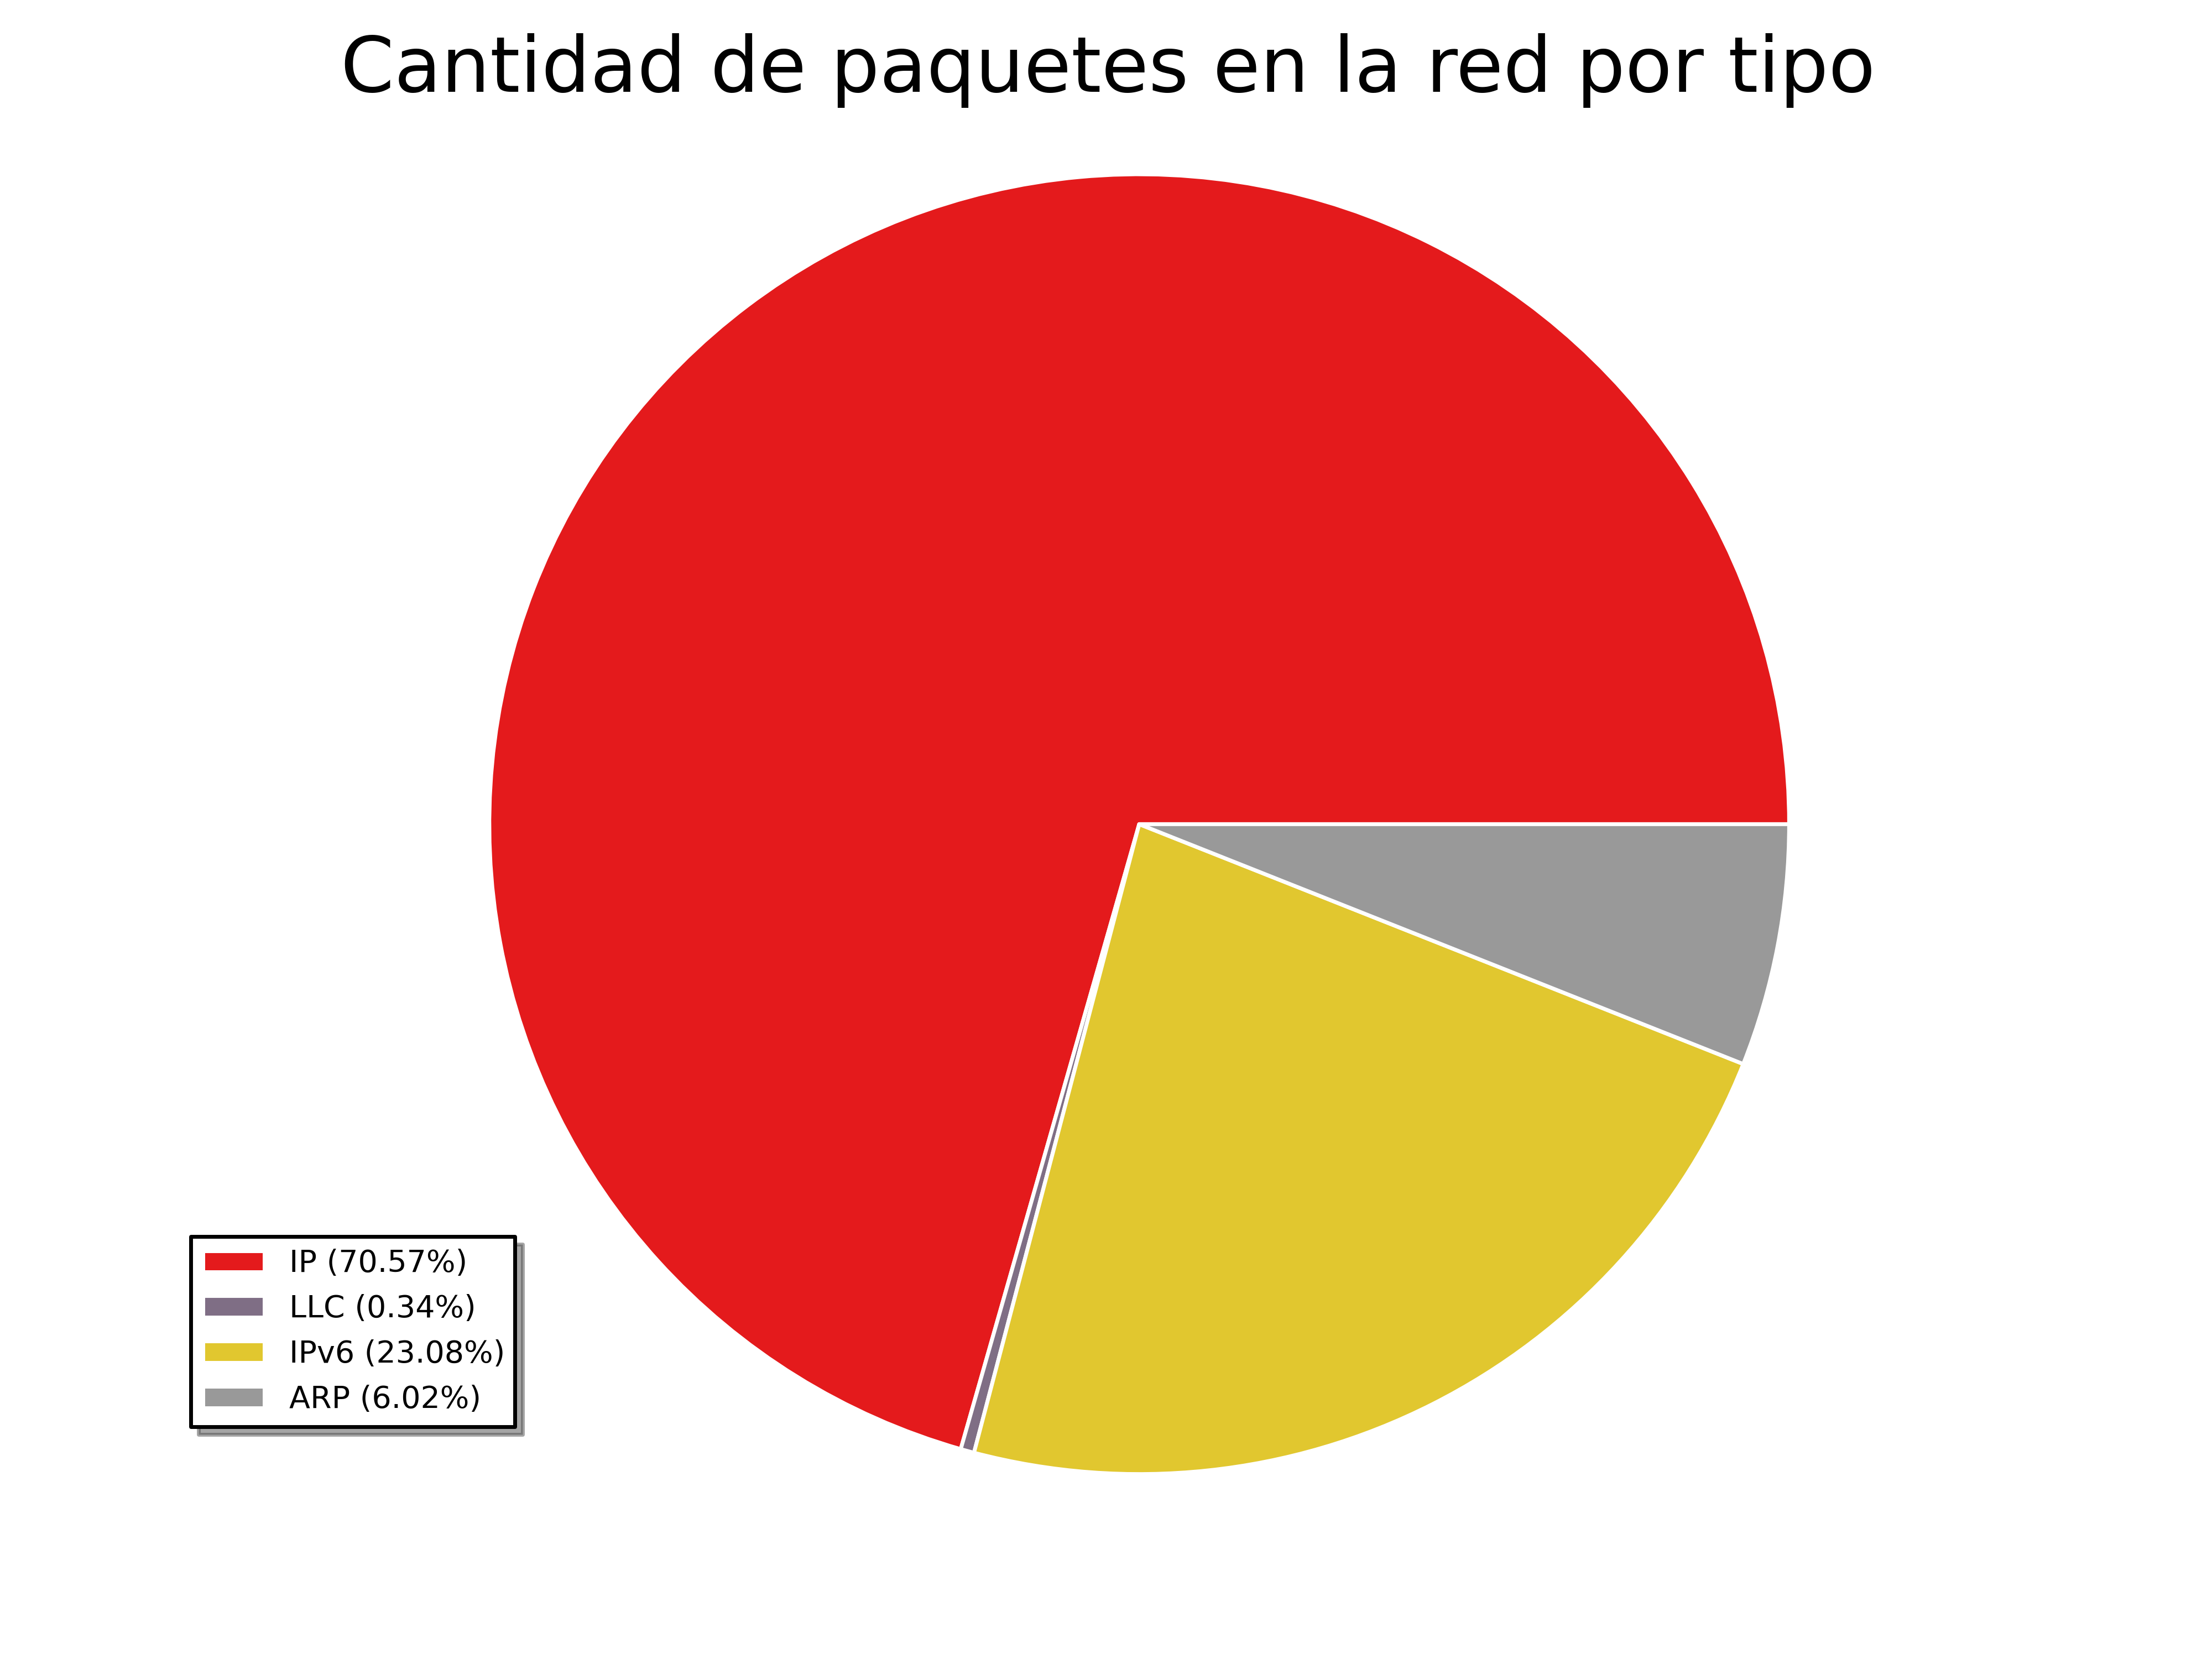
\includegraphics[width=0.7\textwidth]{graficos/red_baufest_pie_type.png}
  \caption{Mi Figura}
  \label{fig:red_baufest_pie_type}
\end{figure}

\begin{figure}[h!]
  \centering
   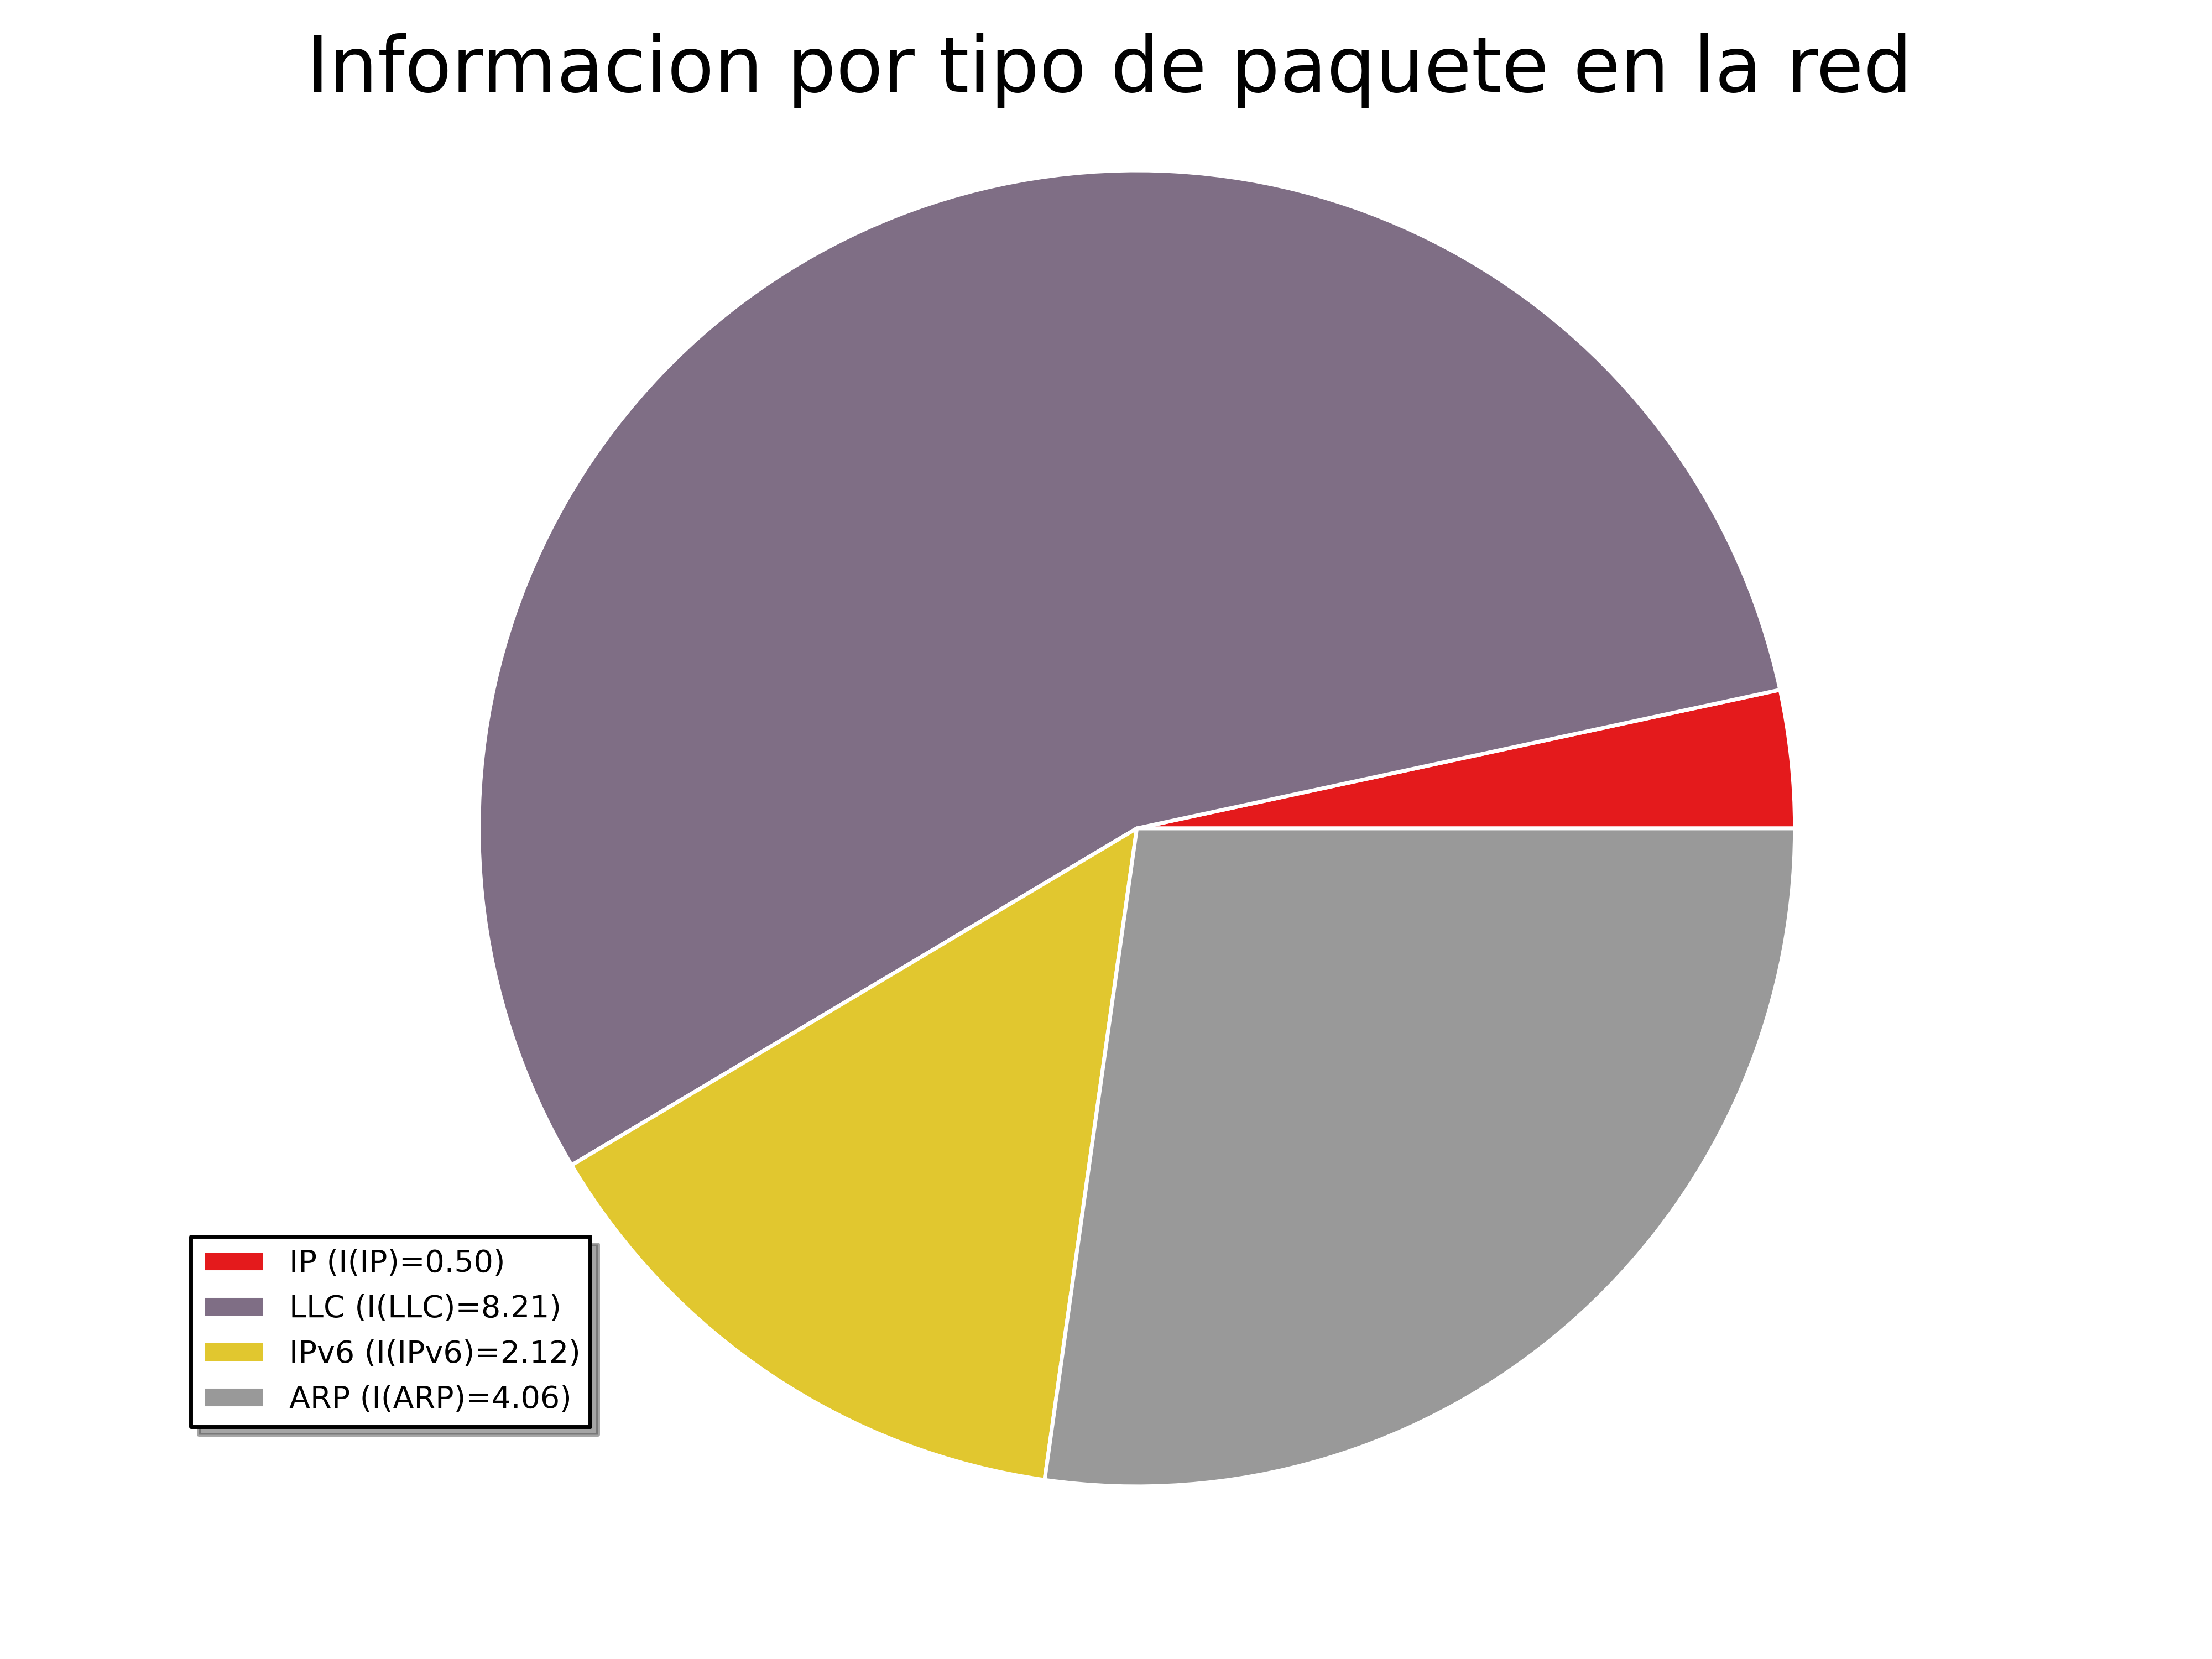
\includegraphics[width=0.7\textwidth]{graficos/red_baufest_pie_type_information.png}
  \caption{Mi Figura}
  \label{fig:red_baufest_pie_type_information}
\end{figure}